\chapter{vSMC: A C++ Library for Parallel SMC}
\label{cha:vSMC: A C++ Library for Parallel SMC}

The \vsmc library \cite{software:VSMC} was developed during the research to
assist the implementation of various \smc and other algorithms, including but
not limited to the implementation of the illustrative and performance
comparison examples in previous chapters. It evolves into a sophisticated \cpp
framework for implementing \smc algorithms on both sequential and parallel
hardware.

A more comprehensive (but also much more technical) tutorial of the library
can be found in \cite{software:VSMC}, part of which is also presented in this
chapter. In this chapter, we provide a higher level overview of the library
structure and usage. Section~\ref{sec:Using the vSMC library} and~\ref{sec:The
  vSMC library} details the usage and structure of the library. In
section~\ref{sec:A minimal example} we use a minimal example to demonstrate
the most basic features of the library. Section~\ref{sec:Beyond the basics}
discusses how one can implement the adaptive algorithms studied in the last
chapter and how the library can assist novel \smc related researches. In the
field of \smc, and computational statistics in general, researchers are
actively developing new algorithms. It is unlikely to have any existing
software to directly provide functionality of the newly developed algorithms.
One of the purpose of \vsmc is to make it easier to develop new \smc related
algorithms on top of the presented framework, and to free researchers from
developing entirely new software to satisfy their particular needs. In
section~\ref{sec:Performance benchmark} we compare the performance of
different parallel programming models that can be used with \vsmc.

It shall be noted that, \vsmc may be more ``developer friendly'' than ``user
friendly''. It does not provide \bugs-like interface for the user. However,
the more proficient one is at \cpp, \vsmc may be used in a more flexible and
productive way than other softwares. There is always a trade-off between easy
of use and the productivity, flexibility and extensibility of a given
software.

The advancement of the Monte Carlo research is tightly related to the
improvement in computer performance and development of various software. In
this section, we review the recent history and state of statistical software
with a particular emphasis on their application for implementation of Monte
Carlo algorithm.

In recent years, there is a new trend in computer technologies. Parallel
computing has become more accessible to many researchers. How to take
advantage of this new trend to develop and implement novel Monte Carlo
algorithms is one of the main purpose of the work presented in this chapter.

\section{The state of softwares for Monte Carlo computing}
\label{sec:The state of software for Monte Carlo computing}

The use of computer for statistical computing and Monte Carlo computing in
particular an be dated as far as back to 1950s. It has seen the most
development

\section{Parallel computing in statistics}
\label{sec:Parallel computing in statistics}

Parallel computing is a form of computation in which many calculations are
carried out simultaneously. It operates on the principle that large problems
can be divided into independent smaller ones and can be solved concurrently
(``in parallel''). Parallelism has been practiced for many years, in the form
of high performance computing. In recent year, it has also become the dominant
paradigm for desktop computing in the form of multicore processor. However,
most of today's popular statistical softwares are written with serialization
as an assumption, meaning that they do not easily take advantage of
contemporary computer architectures.

\subsection{Strategies}
\label{sub:Strategies}

The best overall strategy for \emph{scalable parallelism} is \emph{data
  parallelism} \cite{datapar}. There are various definitions of data
parallelism. Narrower definitions only permit collection-oriented operations,
such as applying the same function to all elements of an array. A wider view
is that the parallelism grows (preferably linearly) as the data size or the
problem size grows. For example, parallelize an vanilla algorithm belongs to
this strategy. As the number of samples increases, one can always use more
parallel computing resources to run the sampler with the same amount of time
without increasing the speed of each computing unit. Note that, here we
ignored issues such as generating random numbers in parallel, which will be
discussed later. In contrast, a \mcmc algorithm is cannot be parallelized in a
scalable way. To obtain better statistical results, often the only way is to
increase the number and iterations, and thus no matter how much parallel
computing resources are available, the computing time will increase without
increasing of the speed of the processors.

The opposite of data parallelism is \emph{functional parallelism}, an approach
that runs different functional parts of a program in parallel. At best,
functional parallelism can improvement the performance. For example, say a
program performs function $f_1,\dots,f_k$, then at best the computing time can
be reduced by $k$-fold through parallelism. In the remaining of this chapter,
we focus on data parallelism.

\subsubsection{Parallel patterns}
\label{ssub:Parallel patterns}

In a more micro level, parallelism can be implemented with different patterns.
In this section, we introduce a few that are particularly related to
statistical computing.

The term \emph{pattern} in computer science, introduced and popularized by
\cite{software:GoF}, is a way of codifying best practices for software
engineering. Instead of discuss different hardware implementations or abstract
classification of parallelism, we found patterns is more useful to
statisticians for reasoning the parallel structure of a given algorithm. This
section is not an exhaustive discussion of parallel patterns. Instead, we
choose some of the most commonly seen in practice, in particular those
particularly relevant to Monte Carlo algorithms.

\paragraph{Map}

This is perhaps the simplest form of parallelism. A function, called
\emph{elemental function}, is replicated for each element of a data collection
concurrently. The elemental function must have no side-effects in order for
the map to be implementable in parallel while achieving deterministic results.
In particular, it cannot modify global data that other instances of that
function depend on.

In \smc algorithm, the updating of particle values is clearly implementable
using a map pattern. The operation of the kernel $K(x_{t-1},x_t)$ depends only
on the history of the particle that it will be used to update, but not other
particles to be updated.

\paragraph{Fork-join}

This pattern lets control flows fork into multiple parallel flows that rejoin
later. The major difference between fork-join and map is that fork-joint does
not necessarily apply the same function on different data. Instead, usually
different functions are applied to different or the same data. There are
different programming models that implement this pattern.  The \openmp's
\cppinline{parallel region} fork control into multiple threads that all
execute the \emph{same} statements and use other constructs to determine which
thread does what. The \cilk's \cppinline{spawn} fork a new thread to execute
the calling function on a new thread and it is later joined with the callee.

The fork-join pattern are often used by programming models to implement other
patterns and is widely used in practice. One example is numerical
integrations, especially for adaptive schemes. Whenever a new segment of the
integral interval is chosen, the program can fork a new thread to compute the
results. And after all segments are computed, the program can join all threads
and sum up the final result.

\paragraph{Reduction}

This pattern uses an associative operator to combine every element in a
collection into a single element. Given the associativity of the operator,
many different orderings are possible and hence multiple threads can be used
to parallelize the computation. This is most often used for parallelization of
computations such as summations.

For example, the computation of \ess, \cess, normalizing of weights, etc., are
all parallelized using the reduction pattern within \vsmc.

\subsubsection{Pipeline}
\label{ssub:Pipeline}

A pipeline connects tasks in a \emph{producer-consumer} relationship. A few
computation units are active at the same time. The first one consume the data,
and produce new data to be used by the second, and so on.

There are several applications of pipeline in Monte Carlo computing. For
example, an \mcmc algorithm often need to compute various convergence
statistics, say $h(X_{0:t})$. Often, this statistic can be written as
$h(X_{0:t}) = h(X_t, h(X_{0:{t-1}}))$. Instead of compute it after all
iterations, one can use one thread to update the \mcmc chain and another one
to compute the statistics, using the pipeline pattern. In this case, the
Markov kernel that update the states is the \emph{producer} and the thread
that update the statistics is the \emph{consumer}.

\subsection{Classes of parallel computers}
\label{sub:Classes of parallel computers}

There are a few types of parallel computers. Here we introduce the four types
of hardware parallelism that are most commonly seen. Parallel computers can be
nested. In a multicore \cpu, each core can perform instruction level
parallelism. On the other hand, a distributed system can be formed by multiple
multicore \cpu.

\subsubsection{Instruction level}
\label{ssub:Instruction level}

Modern \cpu all implement the so called \simd instructions, short for
\emph{single instruction, multiple data}. The \cpu can execute a single
instruction on different data in a single cycle. However, unlike the higher
level parallelism discussed later, \simd often has strict requirement of the
arrangement of the data. In addition, the implementation often requires using
low level assembly language or intrinsics functions.

Though \vsmc does not directly implement this level of parallelism, it can be
used by the user nonetheless. In addition, many operations within \vsmc can be
performed using libraries that are implemented with \simd parallelization,
such as \mkl. Also note that, most modern \cpp compilers also perform \simd
optimizations on simple loop and some of them, such as \clang performs \simd
optimizations for non-loop structures. This kind of optimization is also
called \emph{vectorization}.

\subsubsection{Multicore processors and symmetric multiprocessing}
\label{ssub:Multicore processors and symmetric multiprocessing}

In the late 1990s, computer \cpu are most advanced by increasing the clock
speed. However, this strategy soon hit some bottlenecks, mainly the control of
heat and power. The industry started to develop multicore processors. Each
\cpu has several cores, each running at a modest clock speed. By executing
different threads on different cores, the \cpu can process the same amount of
work with less time without increasing the clock speed.

When a computer has multiple \cpu and each of then has the same speed to
access the memory, the system is often called \emph{symmetric multiprocessing}
(\smp). Most higher end workstations are \smp systems. The programming tools
are usually the same for \smp and multicore processors.

Though multicore processors now sit in a vast majority of consumer and
professional computers, its programming is more difficult than sequential
programming. Parallel programs are more difficult to reasoning and issues such
as data race often cause surprising behaviors of the program. Such issues will
be briefly discussed in section~\ref{sub:Thread-safety and scalability
  considerations}.

The \vsmc library support various \smp programming models. In addition, \vsmc
allows the same user implementation source code to be compiled into different
parallel samplers using different programming models.

\subsubsection{Distributed computing}
\label{ssub:Distributed computing}

Distributed computing usually refers to the form of computing where both
memory and computing processors are spread among computing nodes. It can take
different forms, such as grid and clusters. The \emph{de facto} programming
model for distributed computing is \mpi. This is also supported by \vsmc. In
addition, the library also allows easy integration of \mpi and various \smp
programming models.

\subsubsection{Massive parallel computing}
\label{ssub:Massive parallel computing}

In recent years, there is a new trend of using specialized massive parallel
computing devices, such as \gpu for scientific computing. Modern \gpu often
has hundreds or thousands co-processors. The main difference between \gpu and
\cpu is that, \cpu has more logic control units, and thus is more suited for
general programs. In contrast, \gpu are better at applying the same arithmetic
operations on a collection of data. It performs the best if each computing
units are executing \emph{exactly the same} instructions. In addition, it is
often much more efficient if there are a large amount data to be processed.
Another significant feature of these devices is that they provide much higher
\emph{local} memory bandwidth and can use various techniques to reduce local
data latency than traditional \cpu.

Massive parallel computing is extremely suitable for the \smc algorithms,
which can have a large number of particles, while each of then need to be
updated using the same \mcmc kernel.

There are two major programming models for general purpose \gpu programming
(\gpgpu), Nvidia's \cuda framework and the \opencl standard. The \vsmc library
provides direct support for the \opencl programming model.

\subsection{Importance and limitations of parallel computing}
\label{sub:Importance and limitations of parallel computing}

Parallel computers has been developed for decades. Several recent reasons have
led to increased level of parallel computing in individual, mainstream
personal computers.

\subsubsection{The hardware trend and the cost of computing}
\label{ssub:The hardware trend and the cost of computing}

The most significant one is the hardware trend. From 1973 to 2003, clock rates
of processors increased from 1 MHz to 1 GHz. However, since then there are
little improvement on this front. Now most high end workstations has
processors with clock rates at about 2.5 GHz. However, virtually all
processors produced now have multiple cores. Eight to twelve cores
configurations are common in middle to high end workstations and personal
computers often have at least two cores with quadric configurations more and
more commonly seen, while the clock rates not only remains flat, but also has
the trend of decreasing. These changes are due to various technical
difficulties in increasing the clock rates among other reasons, which we will
not elaborate further here.

Scientists are ever seeking to solving more complex problems, which requires
more computations. To solve larger problems without use significantly longer
computing times, the only way is to use parallelism.

Even for the same problem size, parallelism, whenever possible also has other
benefits apart from reduced computational time. One more important of then is
the power consumption. The power consumption of a \cmos circuit, the dominant
technology used in today's computer, is
\begin{equation}
  P \propto V^2f
\end{equation}
where $V$ is the voltage and $f$ is the frequency. However, the highest
frequency is roughly proportional to the voltage. In other words, the power
consumption is roughly proportional to the \emph{cube} of the frequency.
Therefore, say running two processors, each has half the frequency and doing
the same amount of work with the same computing time, only a quarter of power
will be used.

In summary, parallel computing is much more economic than sequential
computing. In realistic, it means researchers can invest the same or less
amount of funding, yet get more computing work done with the same or less
time.

\subsection{Work-span model and speedup}
\label{sub:Work-span model and speedup}

Unlike sequential computing, the performance of parallel computing is more
difficult to study. In sequential situation, the computational cost can often
be deduced from the algorithms easily. For example, a Monte Carlo algorithm
can use the total number of samples to be generated as a measure of its
computational cost. However, in the case of parallel computing, the total
amount of computation, whether measured as number arithmetic operations or
data operations, cannot reflect the cost in reality. This is due to the fact
that, today's parallel computers is much more cost efficient when more work
are parallelized, for reasons such as power consumption mentioned before.

The study of the performance of parallel programming is usually based on the
work-span model. In this model, tasks form a \emph{direct acyclic graph}
(\dag). A task is ready to run if all of its predecessors in the graph are
done. The basic model ignores communication and memory access costs. It also
assumes the task scheduling is \emph{greedy}, which means that is will never
let a hardware worker idle while there is a task ready to run.

Let $P$ be the number of hardware workers, e.g., cores in multicore processor
and nodes in a cluster, and $T_P$ be the total time of computation. In this
model, $T_1$ is called the \emph{work} of the program and $T_{\infty}$ is
called the span, which is equal to the longest path in the \dag measured in
time, the \emph{critical path}. Because the existence of the critical path,
$T_P \ge T_1/P$. Thus the speedup, defined as $S_P = T_1/T_P$, is bounded,
\begin{equation}
  S_P \le \frac{T_1}{T_1/P} = P
\end{equation}
In addition, assuming that adding processors never slows down the program,
\begin{equation}
  S_P \le T_1/T_{\infty}
\end{equation}
Therefore, the structure of the algorithm determine the maximum speedup it can
obtain.

Implementations on different hardwares often are interested in one of the
three quantities, $T_1$, $T_P$ and $T_{\infty}$. For sequential
implementations clearly $T_1$ is the only one of interest. For multicore and
\smp systems, $T_P$ is of interest for a particular value $P$. $T_{\infty}$ is
previously of less interest, which is only considered as an ideal situation.
However, the recent development on massive parallel computers has made it
close to a reality for many algorithms.

\subsection{Limitations}
\label{sub:Limitations}



\subsection{Challenges of parallel computing for Monte Carlo algorithms}
\label{sub:Challenges of parallel computing for Monte Carlo algorithms}

\subsubsection{Generating random numbers}
\label{ssub:Generating random numbers}

One significant challenge, often well understood yet over sighted by
statisticians in practice is the generating of random numbers in parallel.
Most well known random number generators (\rng) are pseudo-\rng, such as
\textsc{mt19937}. They operates by applying a deterministic function on some
internal state sequentially. That is, given the state $x_t$, the next random
number $x_{t+1}$ is generated by $x_{t+1} = f(x_t)$. The entire sequence is
determined by the state $x_0$, often called the \emph{seed} and the procedure
that initialize the sequence is called \emph{seeding}.

There are many efforts to parallelize pseudo-\rng. The common strategy is that
each thread has its own \rng sequence with a different seed. However, without
proper seeding, it is possible that at some point, part of the sequence of one
thread is exactly the same as another thread. Algorithms that generating
proper seeds often has an order greater than $O(n)$ where $n$ is the number of
threads, and thus its scalability is limited.

One interesting development in recent year is by \cite{Salmon:2011um}. They
took idea from the encryption literature, where for an integer $x$, a number
$y$ is generated through a deterministic, one-to-one mapping, $y = f(x)$. This
function has such a property that, given a collection $\{x_i\}_{i=1}^N$, the
generated collection $\{y_i\}_{i=1}^N$ appears to be random for statistical
use. When implemented in parallel, as long as each thread has different input
sequence $\{x_i\}$, even they are just $\{1,2,\dots\}$, the output will be
legitimate.

The library provided by \cite{Salmon:2011um} has a performance close to
the well known \textsc{mt19937} generator while can be easily parallelized.
And it is used extensively by \vsmc.

\subsubsection{Structures of algorithms}
\label{ssub:Structures of algorithms}

Some algorithms, or part of its structures are unsuitable for parallelization.
This is often due to the dependence among data. For example, the most \mcmc
algorithm cannot be efficiently parallelized. The \smc algorithms, though many
of them can be parallelized easily, in most situations, the resampling step
still cannot be efficiently parallelized. In some situations, resampling only
consumes a small amount of computational time and does not matter much.
However, in some algorithms, the resampling algorithm can be a performance
bottleneck. In addition, requirement of synchronization points (so each
thread has the same view of the weight before and after the resampling step),
can significantly reduce the performance when the computational cost of
updating each particle is not even. In this case, most particles could be
waiting for the new state and weight of a few particles.

These problems cannot be easily solved by the improvement of computers or
software tools. Instead, they require researchers to design algorithms that
are more suitable for the new trend of computer hardware. This is also one of
the reason that population based Monte Carlo algorithms have attracted
considerable attention in recent years. For example, there are recent
development of the particle \mcmc algorithm \cite{Andrieu:2010gc}, which
combines the strength of \mcmc and \smc algorithms and the \smc part can be
parallelized. In particular case of \smc, there are also development on
solving the bottleneck issue of resampling, for example, see
\cite{presampling}.

\subsubsection{Scalability of algorithms}
\label{ssub:Scalability of algorithms}

Many Monte Carlo algorithms enjoys some form of the central limit theorem and
the computational cost is often $O(N)$ where $N$ is the number of samples
(iterations in \mcmc and number of particles in \smc, etc.) In sequential
implementations, this leads to that to get $K$ times the performance (in the
sense of, e.g., $1/K$ times the estimator variance), one can archive that by
investing $K$ times the computational cost.

The situation is more complex in parallelized programs. As we can see in
section~\ref{sec:Performance benchmark}, these programs does not generally
enjoy such a linear relation. The programs often perform more efficiently when
there is a large number of samples in the sense that, the computational time
can be reduced close to linearly by increasing the number of threads. However,
the performance of Monte Carlo algorithms cannot be measured by computational
time along. For example, in the case of the \pmcmc algorithm, to increase the
number of threads leads to increasing the number of \mcmc chains within the
algorithm. As we see in the earlier chapter, such a change can lead to slower
global mixing speed and hence slow down the whole algorithm.

The \smc algorithm, though is more desirable in the sense that increasing
number of particles improve the efficiency of parallelization while the
variance of estimators reduce according to some form of the central limit
theorem. However, given the same computational time, there is still the
trade-off between the number of particles and the number of distributions.
Increasing the former improves the computational efficiency while increasing
the later improves the mixing speed of the forward Markov kernel.

Nonetheless, among all algorithms studied in this thesis, \smc is perhaps the
most scalable one.

\section{An overview of C++ and template metaprogramming}
\label{sec:An overview of C++ and template metaprogramming}

\cpp is a static strong type language. It requires the user to declare
variables, functions, and most other kinds of entities using specific types.
However, a lot of code looks the same for different types. Especially for
implementation of algorithms, including but not limited to Monte Carlo
computing. The \cpp template technique allows one to write generic code to
solve a class of problems, while the involved types can be seamlessly replaced
at compile time. In this section, we briefly introduce the basic knowledges of
\cpp template, to ease the reading of what follows. We assume the reader has
at least some working knowledge of \cpp, including concepts such as
object-oriented programming.

\subsection{Function template}
\label{sub:Function template}

The following lines define a simple function template,
\cppfile{code/function_template_def.cpp}
This template definition specifies a \emph{family} of functions that returns
the maximum of two values, which are passed as function parameters
\cppinline{a} and \cppinline{b}. They type of these parameters is left open as
\emph{template parameter} \cppinline{T}. Here we see one form of the template
parameter \cppinline{typename T}. A generic type is declared in this form.
There are two other forms, non-type parameter and template template parameter.
Non-type parameter can be any compile time constant expression, such as
integer literates. Template template parameter can use a class template name
as a parameter, which is a more complex topic. All three forms are used in
\vsmc, and we will see examples of the usage of them in context.

In this template definition, the assumption about \cppinline{T} is that the
operator \cppinline{<} is properly defined. The actual types are deduced at
compile time when the function template is used. A detailed account of this
topic is beyond the scope of this section. However, below we give some correct
and incorrect examples of the usage of this template.
\cppfile{code/function_template_usage.cpp}

\subsection{Class template}
\label{sub:Class template}

Class template is similar to function template, yet somehow simpler. A class
template define a family of classes. For example,
\cppfile{code/class_template_def.cpp}
defines a \cppinline{Stack} class template. For simplicity, some edge cases
and exceptional situations such as calling \cppinline{top} on an empty
\cppinline{Stack} is not handled here. This class template can be used as the
following,
\cppfile{code/class_template_usage.cpp}
As we can see, to use a class template, one \emph{explicitly} supply the type
of the template parameter. Unlike function template, there is no template
parameter deduction here.

\subsection{Specialization}
\label{sub:Specialization}

There are many more in-depths topics and features of \cpp template that we
have note discussed in this section, due to the limit of the scope. There are
books devoted entirely to such topics \cite{cpptemplate, moderncpp}. One
feature used extensively in the \vsmc library is \emph{specialization},
especially specialization of class template. Specialization allows one to
provide special definition of a class template for one particular type of the
template parameter. And hence it allows one to manipulate types at compile
time.

One simple example is the following,
\cppfile{code/class_template_spec.cpp}
The first definition of the class \cppinline{SizeType} is generic and the
second is its specialization for type \cppinline{SomeSpecialType}. The class
\cppinline{Sampler}, which uses the type \cppinline{size_type}, will define
this type to be \cppinline{std::size_t}. However, for some special type
\cppinline{SomeSpecialType}, this type will be defined as \cppinline{int}.

There are more advanced usages of template specialization. These are used
extensively in \vsmc to provide extensibility. The key observation from the
above example is that, template specialization provides special behavior for
some type in addition to the generic behavior to other types. The ability to
programming on types of \cpp templates leads to the popularity of \cpp
template metaprogramming in the past decade. See \cite{moderncpp} for some
advanced techniques.

\section{Using the vSMC library}
\label{sec:Using the vSMC library}

\subsection{Overview}

The \vsmc library makes use of \cpp's template generic programming to
implement general \smc algorithms. This library is formed by a few major
modules listed below. Some features not included in these modules are
introduced later in context.
\begin{description}
  \item[Core] The highest level of abstraction of \smc samplers. Users
    interact with classes defined within this module to create and manipulate
    general \smc samplers. Classes in this module include \cppinline{Sampler},
    \cppinline{Particle} and others. These classes use user defined callback
    functions or callable objects, such as functors, to perform problem
    specific operations, such as updating particle values and weights. This
    module is documented in Section~\ref{sub:Core module}.
  \item[Symmetric Multiprocessing (\smp)] This is the form of computing most
    people use everyday, including multiprocessor workstations, multicore
    desktops and laptops. Classes within this module make it possible to write
    generic operations which manipulate a single particle that can be applied
    either sequentially or in parallel through various parallel programming
    models. A method defined through classes of this module can be used by
    \cppinline{Sampler} as callback objects. This module is documented in
    section~\ref{sub:SMP module}.
  \item[Message Passing Interface] \mpi is the \emph{de facto} standard for
    parallel programming on distributed memory architectures. This module
    enables users to adapt implementations of algorithms written for the \smp
    module such that the same sampler can be parallelized using \mpi. In
    addition, when used with the \smp module, it allows easy implementation of
    hybrid parallelization such as \mpi/\openmp.
  \item[\opencl] This module is similar to the two above except it eases the
    parallelization through \opencl, such as for the purpose of General
    Purpose \gpu Programming (\gpgpu). \opencl is a framework for writing
    programs that can be execute across heterogeneous platforms. \opencl
    programs can run on either \cpu or \gpu.
\end{description}
We will introduce the core and \smp modules in detail. The other two will
requires substantial knowledge of the underlying programming models, and it is
beyond the scope of this chapter to give them proper introduction. However,
examples and performance comparison will be given in context later.

\subsection{Obtaining and installation}

\vsmc is a header only library. There is practically no installation step. The
library can be downloaded from \url{http://zhouyan.github.io/vSMC/vSMC.zip}.
After downloading and unpacking, one can start using \vsmc by ensuring that
the compiler can find the headers inside the \cppinline{include} directory. To
permanently install the library in a system directory, one can simply copy the
contents of the \cppinline{include} directory to an appropriate place.

Alternatively, one can use the \cmake (version~2.8 or later) configuration
script and obtain the source by \git. On a Unix-like system (such as Mac OS X,
BSD, Linux and others),
\begin{shcode}
git clone git://github.com/zhouyan/vSMC.git
cd vSMC
git submodule init
git submodule update
mkdir build
cd build
cmake .. -DCMAKE_BUILD_TYPE=Release
make install
\end{shcode}

\subsection{Documentation}

To build the reference manual, one needs Doxygen (version~1.8.3 or later).
Continuing the last step (still in the \cppinline{build} directory), invoking
\shinline{make docs} will create a \shinline{doc} directory inside
\shinline{build}, which contains the \html references. Alternatively the
reference manual can also be found on
\url{http://zhouyan.github.io/vSMC/doc/html/index.html}. It is beyond the
scope of this chapter to document every feature of the \vsmc library. In many
places we will refer to this reference manual for further information.

\subsection{Third-party dependencies}

\vsmc uses \random \cite{Salmon:2011um} counter-based \rng for random number
generating. For an \smc sampler with $N$ particles, \vsmc constructs $N$
(statistically) independent \rng streams. It is possible to use millions of
such streams without a huge memory footprint or other performance penalties.
Since each particle has its own independent \rng stream, it frees users from
many thread-safety and statistical independence considerations. It is highly
recommended that the users install this library. Within \vsmc, these \rng
streams are wrapped under \cppoo{} \rng engines, and can be replaced by other
compatible \rng engines seamlessly. Users only need to be familiar with
classes defined in \cppoo{} \cppinline{<random>} or their Boost equivalents to
use these \rng streams. See the documentation of the corresponding libraries
for details, as well as examples in Section~\ref{sec:A minimal example}.

The other third-party dependency is the Boost library. Version~1.49 or later
is required. However, this is actually optional provided that proper \cppoo
features are available in the standard library, for example using \clang with
\libcpp The \cppoo headers of concern are \cppinline{<functional>} and
\cppinline{<random>}. To instruct \vsmc to use the standard library headers
instead of falling back to the Boost library, one needs to define the
configuration macros before including any \vsmc headers. For example,
\begin{shcode}
clang++ -std=c++11 -stdlib=lib++     \
    -DVSMC_HAS_CXX11LIB_FUNCTIONAL=1  \
    -DVSMC_HAS_CXX11LIB_RANDOM=1      \
    -o prog prog.cpp
\end{shcode}
tells the library to use \cppoo{} \cppinline{<functional>} and
\cppinline{<random>}. The availability of these headers are also checked by
the \cmake configuration script.

\subsection{Compiler support}

\vsmc has been tested with recent versions of \clang, \gcc, \icpc and \msvc.
\vsmc can optionally use some \cppoo features to improve performance and
usability. In particular, as mentioned before, \vsmc can use \cppoo standard
libraries instead of the Boost library. At the time of writing, \clang with
\libcpp has the most comprehensive support of \cppoo with respect to standard
compliant and feature completion. \gcc~4.8, \msvc~2012 and \icpc~2013 also
have very good \cppoo support. Note that, provided the Boost library is
available, all \cppoo language and library features are optional. \vsmc can be
used with any \cppne conforming compilers.

\section{The vSMC library}
\label{sec:The vSMC library}

\subsection{Core module}
\label{sub:Core module}

The core module abstracts general \smc samplers. \smc samplers can be viewed
as formed by a few concepts regardless of the specific problems. The following
is a list of the most commonly seen components of \smc samplers and their
corresponding \vsmc abstractions. Here and in the remaining of this chapter,
unless stated otherwise, all documented classes resides in the
\cppinline{vsmc} namespace.
\begin{itemize}
  \item A collection of all particle state values, namely
    $\{X_t^{(i)}\}_{i=1}^N$. In \vsmc, users need to define a class, say
    \cppinline{T}, to abstract this concept. We refer to this as the
    \emph{value collection}. We will slightly abuse the generic name
    \cppinline{T} in this chapter. Whenever a template parameter is mentioned
    with the name \cppinline{T}, it always refers to such a value collection
    type unless stated otherwise.
  \item A collection of all particle state values and their associated
    weights. This is abstracted by a \cppinline{Particle<T>} object. We refer
    to this as the \emph{particle collection}. A \cppinline{Particle<T>}
    object has three primary sub-objects. One is the above type \cppinline{T}
    value collection object. Another is an object that abstracts weights
    $\{W_t^{(i)}\}_{i=1}^N$. By default this is a \cppinline{WeightSet}
    object. The last is a collection of \rng streams, one for each particle.
    By default this is an \cppinline{RngSet} object.
  \item Operations that perform tasks common to all samplers to these
    particles, such as resampling. These are the member functions of
    \cppinline{Particle<T>}.
  \item A sampler that updates the particles (state values and weights) using
    user defined callbacks. This is a \cppinline{Sampler<T>} object.
  \item Monitors that record the importance sampling estimates of certain
    functions defined for the values when the sampler iterates. These are
    \cppinline{Monitor<T>} objects. A monitor for the estimates of $E[h(X_t)]$
    computes $h(X_t^{(i)})$ for each $i = 1,\dots,N$. The function value
    $h(X_t)$ is allowed to be a vector.
\end{itemize}
Note that within the core module, all operations are applied to
\cppinline{Particle<T>} objects, that is $\{W_t^{(i)},X_t^{(i)}\}_{i=1}^N$,
instead of a single particle. Later we will see how to write operations that
can be applied to individual particles and can be parallelized easily.

\subsubsection{Program structures}
\label{ssub:Program structures}

A \vsmc program usually consists of the following tasks.
\begin{itemize}
  \item Define a value collection type \cppinline{T}.
  \item Constructing a \cppinline{Sampler<T>} object.
  \item Configure the behavior of initialization and updating by adding
    callable objects to the sampler object.
  \item Optionally add monitors.
  \item Initialize and iterate the sampler.
  \item Retrieve the outputs, estimates and other informations.
\end{itemize}
In this section we document how to implement each of these tasks. Within the
\vsmc library, all public classes, namespaces and free functions, are declared
in the namespace \cppinline{vsmc}.

\subsubsection{The value collection}
\label{ssub:The value collection}

The template parameter \cppinline{T} is a user defined type that abstracts the
value collection. \vsmc does not restrict how the values shall be actually
stored. They can be stored in memory, spread among nodes of a cluster, in \gpu
memory or even in a database. However this kind of flexibility comes with a
small price. The value collection does need to fulfill two requirements. We
will see later that for most common usage, \vsmc provides readily usable
implementations, on top of which users can create problem specific classes.

First, the value collection class \cppinline{T} has to provide a constructor
of the form
\begin{cppcode}
T (SizeType N)
\end{cppcode}
where \cppinline{SizeType} is some integer type. Since \vsmc allows one to
allocate the states in any way suitable, one needs to provide this constructor
which \cppinline{Particle<T>} can use to allocate them.

Second, the class has to provide a member function named \cppinline{copy} that
copies each particle according to replication numbers given by a resampling
algorithm. For the same reason as above \vsmc has no way to know how it can
extract and copy a single particle when it is doing the resampling. The
signature of this member function may look like
\begin{cppcode}
template <typename SizeType>
void copy (std::size_t N, const SizeType *copy_from);
\end{cppcode}
The pointer \cppinline{copy_from} points to an array that has $N$ elements,
where $N$ is the number of particles. After calling this member function, the
value of particle \cppinline{i} shall be copied from the particle \cppinline{j
  = copy_from[i]}. In other words, particle \cppinline{i} is a child of
particle \cppinline{copy_from[i]}, or \cppinline{copy_from[i]} is the parent
of particle \cppinline{i}. If a particle \cppinline{j} shall remain itself,
then \cppinline{copy_from[j] == j}. How the values are actually copied is user
defined. Note that, the member function can take other forms, as usual when
using \cpp template generic programming. The actual type of the pointer
\cppinline{copy_from}, \cppinline{SizeType}, is
\cppinline{Particle<T>::size_type}, which depends on the type \cppinline{T}.
For example, define the member function as the following is also allowed,
\begin{cppcode}
void copy (int N, const std::size_t *copy_from);
\end{cppcode}
provided that \cppinline{Particle<T>::size_type} is indeed
\cppinline{std::size_t}. However, writing it as a member function template
releases the users from finding the actual type of pointer
\cppinline{copy_from} and the sometimes troubling forward declaration issues.
Will not elaborate such more technical issues further.

\subsubsection{Constructing a sampler}
\label{ssub:Constructing a sampler}

Once the value collection class \cppinline{T} is defined. One can start
constructing \smc samplers. For example, the following line creates a sampler
with $N$ particles
\begin{cppcode}
Sampler<T> sampler(N);
\end{cppcode}
The number of particles is the only mandatory argument of the constructor.
There are two optional parameters. The complete signature of the constructor
is,
\cppfile{code/sampler_constructor.cpp}
The \cppinline{scheme} parameter is self-explanatory. \vsmc provides a few
built-in resampling schemes; see the reference manual for a list of them. User
defined resampling algorithms can also be used. See the reference manual for
details. The \cppinline{threshold} is the threshold of $\ess/N$ below which a
resampling will be performed. It is obvious that if
$\text{\cppinline{threshold}}\ge1$ then resampling will be performed at each
iteration. If $\text{\cppinline{threshold}}\le0$ then resampling will never be
performed. Both parameters can be changed later. However the size of the
sampler can never be changed after the construction.

\subsubsection{Initialization and updating}
\label{ssub:Initialization and updating}

All the callable objects that initialize, move and weight the particle
collection can be added to a sampler through a set of member functions. All
these objects operate on the \cppinline{Particle<T>} object. Because \vsmc
allows one to manipulate the particle collection as a whole, in principle many
kinds of parallelization are possible.

To set an initialization method, one need to implement a function with the
following signature,
\cppfile{code/init_function.cpp}
or a class with \cppinline{operator()} properly defined, such as
\cppfile{code/init_class.cpp}
They can be added to the sampler through
\begin{cppcode}
sampler.init(init_func);
\end{cppcode}
or
\begin{cppcode}
sampler.init(init_class());
\end{cppcode}
respectively. \cppoo{} \cppinline{std::function} or its Boost equivalent
\cppinline{boost::function} can also be used. For example,
\cppfile{code/init_obj.cpp}

The addition of updating methods is more flexible. There are two kinds of
updating methods. One is simply called \cppinline{move} in \vsmc, and is
performed before the possible resampling at each iteration. These moves
usually perform the updating of the weights among other tasks. The other is
called \cppinline{mcmc}, and is performed after the possible resampling. They
are often \mcmc type moves. Multiple \cppinline{move}'s or \cppinline{mcmc}'s
are also allowed. In fact a \vsmc sampler consists of a queue of
\cppinline{move}'s and a queue of \cppinline{mcmc}'s. The \cppinline{move}'s
in the queue can be changed through \cppinline{Sampler<T>::move},
\cppfile{code/sampler_move.cpp}
If \cppinline{append == true} then \cppinline{new_move} is appended to the
existing (possibly empty) queue. Otherwise, the existing queue is cleared and
\cppinline{new_move} is added. The member function returns a reference to the
updated sampler. For example, the following move,
\begin{cppcode}
std::size_t move_func (std::size_t iter, Particle<T> &particle);
\end{cppcode}
can be added to a sampler by
\begin{cppcode}
sampler.move(move_func, false);
\end{cppcode}
This will clear the (possibly empty) existing queue of \cppinline{move}'s and
set a new one. To add multiple moves into the queue,
\begin{cppcode}
sampler.move(move1, true).move(move2, true).move(move3, true);
\end{cppcode}
Objects of class type with \cppinline{operator()} properly defined can also be
used, similarly to the initialization method. The queue of \cppinline{mcmc}'s
can be used similarly. See the reference manual for other methods that can be
used to manipulate these two queues.

In principle, one can combine all moves into a single move. However, sometimes
it is more natural to think of a queue of moves. For instance, if a
multi-block Metropolis random walk consists of kernels $K_1$ and $K_2$, then
one can implement each of them as functions, say \cppinline{mcmc_k1} and
\cppinline{mcmc_k2}, and add them to the sampler sequentially,
\begin{cppcode}
sampler.mcmc(mcmc_k1, true).mcmc(mcmc_k2, true);
\end{cppcode}
Then at each iteration, they will be applied to the particle collection
sequentially in the order in which they are added.

\subsubsection{Running the algorithm, monitoring and outputs}
\label{ssub:Running the algorithm, monitoring and outputs}

Having set all the operations, one can initialize and iterate the sampler by
calling
\begin{cppcode}
sampler.initialize((void *)param);
sampler.iterate(iter_num);
\end{cppcode}
The \cppinline{param} argument to \cppinline{initialize} is optional, with
\cppinline{NULL} as its default. This parameter is passed to the user defined
\cppinline{init_func}. The \cppinline{iter_num} argument to
\cppinline{iterate} is also optional; the default is $1$.

Before initializing the sampler or after a certain time point, one can add
monitors to the sampler. The concept is similar to \bugs's \cppinline{monitor}
statement, except it does not monitor the individual values but rather the
importance sampling estimates. Consider approximating $\Exp[h(X_t)]$, where
$h(X_t) = (h_1(X_t),\dots,h_m(X_t))$ is an $m$-vector function. The importance
sampling estimate can be obtained by $AW$ where $A$ is an $N$ by $m$ matrix
where $A(i,j) = h_j(X_t^{(i)})$ and $W = (W_t^{(i)},\dots,W_t^{(N)})^T$ is the
$N$-vector of normalized weights. To compute this importance sampling
estimate, one need to define the following evaluation function (or a class
with \cppinline{operator()} properly defined),
\cppfile{code/monitor_eval.cpp}
and add it to the sampler by calling,
\begin{cppcode}
sampler.monitor("variable.name", m, monitor_eval);
\end{cppcode}
When the function \cppinline{monitor_eval} is called, \cppinline{iter} is the
iteration number of the sampler, \cppinline{m} is the same value as the one
the user passed to \cppinline{Sampler<T>::monitor}; and thus one does not need
global variable or other similar techniques to access this value. The output
pointer \cppinline{res} points to an $N \times m$ output array of row major
order. That is, after the calling of the function,
\cppinline{res[i * dim + j]} shall be $h_j(X_t^{(i)})$.

After each iteration of the sampler, the importance sampling estimate will be
computed automatically. See the reference manual for various ways to retrieve
the results. Usually it is sufficient to output the sampler by
\begin{cppcode}
std::ofstream output("file.name");
output << sampler << std::endl;
\end{cppcode}
where the output file will contain the importance sampling estimates among
other things. Alternatively, one can use the \cppinline{Monitor<T>::record}
member function to access specific historical results. See the reference
manual for details of various overloaded version of this member function.

A reference to the value collection \cppinline{T} object can be retrieved
through the \cppinline{Particle<T>::value} member function. The weights
through a weight set object, which by default is of type
\cppinline{WeightSet}. The \cppinline{Particle<T>::weight_set} member function
returns a reference to this weigh set object. A user defined weight set class
that abstracts $\{W_t^{(i)}\}_{i=1}^N$ can also be used. The details involve
some more advanced \cpp template techniques and are documented in the
reference manual. One possible reason for replacing the default is to provide
special memory management of the weight set. For example, the \mpi module
provides a special weight set class that manages weights across multiple nodes
and perform proper normalization, computation of \ess, and other tasks.

The default \cppinline{WeightSet} object provides some ways to retrieve
weights. Here we document some of the most commonly used. See the reference
manual for details of others. The weights can be accessed one by one, for
example,
\begin{cppcode}
Particle<T> &particle = sampler.particle();
double w_i     = particle.weight_set().weight(i);
double log_w_i = particle.weight_set().log_weight(i);
\end{cppcode}
One can also read all weights into a container, for example,
\begin{cppcode}
std::vector<double> w(particle.size());
particle.weight_set().read_weight(w.begin());
double *lw = new double[particle.size()];
particle.weight_set().read_log_weight(lw);
\end{cppcode}
Note that these member functions accept general output iterators.

\subsubsection{Implementing initialization and updating}
\label{ssub:Implementing initialization and updating}

So far we have only discussed how to add initialization and updating objects
to a sampler. To actually implement them, one writes callable objects that
operate on the \cppinline{Particle<T>} object. For example, a move can be
implemented through the following function as mentioned before,
\begin{cppcode}
std::size_t move_func (std::size_t iter, Particle<T> &particle);
\end{cppcode}
Inside the body of this function, one can change the value by manipulating the
object through the reference returned by \cppinline{particle.value()}.

When using the default weight set class, the weights can be updated through a
set of member functions of \cppinline{WeightSet}. For example,
\begin{cppcode}
std::vector<double> weight(particle.size());
particle.weight_set().set_equal_weight();
particle.weight_set().set_weight(weight.begin());
particle.weight_set().mul_weight(weight.begin());
particle.weight_set().set_log_weight(weight.begin());
particle.weight_set().add_log_weight(weight.begin());
\end{cppcode}
The \cppinline{set_equal_weight} member function sets all weights to be equal.
Similarly, the \cppinline{set_weight} and \cppinline{set_log_weight} member
functions set the values of weights and logarithm weights, respectively. And
the \cppinline{mul_weight} and \cppinline{add_log_weight} member functions
multiply the weights or add to the logarithm weights by the given values,
respectively. All these member functions accept general input iterators as
their arguments.

One important thing to note is that, whenever one of these member functions is
called, both the weights and logarithm weights will be re-calculated,
normalized, and the \ess will be updated. The reason for not allowing changing
a single particle's weight is that, in a multi-threading environment, it is
possible for one to change one weight in one thread, and obtain another in
another thread without proper normalizing. Conceptually, changing one weight
actually changes all weights.

\subsubsection{Generating random numbers}
\label{ssub:Generating random numbers}

The \cppinline{Particle<T>} object has a sub-object, a collection of \rng
engines that can be used with \cppoo{} \cppinline{<random>} or Boost
distributions. For each particle \cppinline{i}, one can obtain an engine that
produces an \rng stream independent of others by
\begin{cppcode}
particle.rng(i);
\end{cppcode}
To generate distribution random variates, one can use the
\cppoo{} \cppinline{<random>} library. For example,
\begin{cppcode}
std::normal_distribution<double> rnorm(mean, sd);
double r = rnorm(particle.rng(i));
\end{cppcode}
or use the Boost library,
\begin{cppcode}
boost::random::normal_distribution<double> rnorm(mean, sd);
double r = rnorm(particle.rng(i));
\end{cppcode}
\vsmc itself also makes use of \cppoo{} \cppinline{<random>} or Boost
depending on the value of the configuration macro
\cppinline{VSMC_HAS_CXX11LIB_RANDOM}. Though the user is free to choose which
one to use in their own code, there is a convenient alternative. For each
class defined in \cppoo{} \cppinline{<random>}, it is imported to the
\cppinline{vsmc::cxx11} namespace. Therefore one can use
\begin{cppcode}
cxx11::normal_distribution<double> rnorm(mean, sd);
\end{cppcode}
while the underlying implementation of \cppinline{normal_distribution} can be
either \cppoo standard library or Boost. The benefit is that if one needs to
develop on multiple platforms, and only some of them support \cppoo and some
of them have the Boost library, then only the configure macro
\cppinline{VSMC_HAS_CXX11LIB_RANDOM} needs to be changed. This can be
configured through \cmake and other build systems. Of course, one can also use
an entirely different \rng system than those provided by \vsmc.

\subsection{SMP module}
\label{sub:SMP module}

\subsubsection{The value collection template}
\label{ssub:The value collection template}

Many typical problems' value collections can be viewed as a matrix of certain
type. For example, a simple particle filter whose state is a vector of length
\cppinline{Dim} and type \cppinline{double} can be viewed as an $N$ by
\cppinline{Dim} matrix where $N$ is the number of particles. A
trans-dimensional problem can use an $N$ by $1$ matrix whose type is a user
defined class, say \cppinline{StateType}. For this kind of problems, \vsmc
provide a class template
\begin{cppcode}
template <MatrixOrder Order, std::size_t Dim, typename StateType>
class StateMatrix;
\end{cppcode}
which provides the constructor and the \cppinline{copy} member function
required by the core module interface, as well as methods for accessing
individual values. The first template parameter (possible value
\cppinline{RowMajor} or \cppinline{ColMajor}) specifies how the values are
ordered in memory. Usually one shall choose \cppinline{RowMajor} to optimize
data access. The second template parameter is the number of variables, an
integer value no less than $1$ or the special value \cppinline{Dynamic}, in
which case \cppinline{StateMatrix} provides a member function
\cppinline{resize_dim} such that the number of variables can be changed at
runtime. The third template parameter is the type of the state values.

Each particle's state is thus a vector of length \cppinline{Dim}, indexed from
\cppinline{0} to \cppinline{Dim - 1}. To obtain the value at position
\cppinline{pos} of the vector of particle \cppinline{i}, one can use one of
the following member functions,
\begin{cppcode}
StateBase<RowMajor, Dim, StateType> value(N);
StateType val = value.state(i, pos);
StateType val = value.state(i, Position<Pos>());
StateType val = value.state<Pos>(i);
\end{cppcode}
where \cppinline{Pos} is a compile time constant expression whose value is the
same as \cppinline{pos}, assuming the position is known at compile time. One
can also read all values. To read the variable at position \cppinline{pos},
\begin{cppcode}
std::vector<StateType> vec(value.size());
value.read_state(pos, vec.begin());
\end{cppcode}
Or one can read all values through an iterator,
\begin{cppcode}
std::vector<StateType> mat(Dim * value.size());
value.read_state_matrix(ColMajor, mat.first());
\end{cppcode}
Alternatively, one can also read all values through an iterator which points
to iterators,
\cppfile{code/state_matrix_read.cpp}

If the compiler support \cppoo{} \cppinline{<tuple>}, \vsmc also provides a
\cppinline{StateTuple} class template, which is similar to
\cppinline{StateMatrix} except that the types of values do not have to be the
same for each variable. This is similar to \rlang's \cppinline{data.frame}.
For example, suppose each particle's state is formed by two
\cppinline{double}'s, an \cppinline{int} and a user defined type
\cppinline{StateType}, then the following constructs a value collection using
\cppinline{StateTuple},
\begin{cppcode}
StateTuple<ColMajor, double, double, int, StateType> value(N);
\end{cppcode}
And there are a few ways to access the state values, similar to
\cppinline{StateMatrix},
\begin{cppcode}
double x0 = value.state(i, Position<0>());
int x2 = value.state<2>(i);
std::vector<StateType> vec(value.size());
state.read_state(Position<3>(), vec.begin());
\end{cppcode}
See the reference manual for details.

\subsubsection{A single particle}
\label{ssub:A single particle}

For a \cppinline{Particle<T>} object, one can construct a
\cppinline{SingleParticle<T>} object that abstracts one of the particle from
the collection. For example,
\begin{cppcode}
Particle<T> particle(N);
SingleParticle<T> sp(i, &particle);
\end{cppcode}
create a \cppinline{SingleParticle<T>} object corresponding to the particle at
position \cppinline{i}. There are a few member functions of
\cppinline{SingleParticle<T>} that makes access to individual particles easier
than through the interface of \cppinline{Particle<T>}. Firt
\cppinline{sp.id()} returns the value of the argument \cppinline{i} in the
above code that created this \cppinline{SingleParticle<T>} object. In
addition, \cppinline{sp.rng()} is equivalent to \cppinline{particle.rng(i)}.
Also \cppinline{sp.particle()} returns a constant reference to the
\cppinline{Particle<T>} object. And \cppinline{sp.particle_ptr()} returns a
pointer to such a constant \cppinline{Particle<T>} object. Note that, one
cannot get write access to a \cppinline{Particle<T>} object through interface
of \cppinline{SingleParticle<T>}. Instead, one can only get write access to a
single particle. For example, If \cppinline{T} is a \cppinline{StateMatrix}
instantiation or its derived class, then \cppinline{sp.state(pos)} is
equivalent to \cppinline{particle.value().state(i, pos)} and the reference it
returns is mutable. See the reference manual for more informations on the
interface of the \cppinline{SingleParticle} class template. Note that, these
\cppinline{SingleParticle<T>} objects are usually not constructed by users,
but rather by the libraries' other classes in the \smp module, and passed to
user defined functions, as we will see very soon.

\subsubsection{Sequential and parallel implementations}
\label{ssub:Sequential and parallel implementations}

Once we have the \cppinline{SingleParticle<T>} concept, we are ready to
introduce how to write implementations of \smc algorithms that manipulate a
single particle and can be applied to all particles in parallel or
sequentially. For sequential implementations, this can be done through five
base classes,
\begin{cppcode}
template <typename BaseState> class StateSEQ;
template <typename T, typename D = Virtual> class InitializeSEQ;
template <typename T, typename D = Virtual> class MoveSEQ;
template <typename T, typename D = Virtual> class MonitorEvalSEQ;
template <typename T, typename D = Virtual> class PathEvalSEQ;
\end{cppcode}
The template parameter \cppinline{BaseState} needs to satisfy the general
value collection requirements in addition to a \cppinline{copy_particle}
member function, for example, \cppinline{StateMatrix}. Other base classes
expect \cppinline{T} to satisfy general value collection requirements. The
details of all these class templates can be found in the reference manual.
Here we use the \cppinline{MoveSEQ<T>} class as an example to illustrate their
usage. Recall that \cppinline{Sampler<T>} expect a callable object which has
the following signature as a move,
\begin{cppcode}
std::size_t move_func (std::size_t iter, Particle<T> &particle);
\end{cppcode}
For the purpose of illustration, the type \cppinline{T} is defined as,
\begin{cppcode}
typedef StateMatrix<RowMajor, 1, double> T;
\end{cppcode}
Here is a typical example of implementation of such a function,
\cppfile{code/move_func.cpp}
where \cppinline{cal_inc_weight} is some function that calculates the
logarithm incremental weights. As we see, there are three main parts of a
typical move. First, we allocate a vector \cppinline{inc_weight}. Second, we
generate normal random variates for each particle and calculate the
incremental weights. This is done through a \cppinline{for} loop. Third, we
add the logarithm incremental weights. The first and the third are
\emph{global} operations while the second is \emph{local}. The first and the
third are often optional and absent. The local operation is also usually the
most computational intensive part of \smc algorithms and can benefit the most
from parallelizations.

With \cppinline{MoveSEQ<T>}, which defines the \cppinline{operator()} as
required by the core module interface, one can derive from this class,
\begin{cppcode}
std::size_t operator() (std::size_t iter, Particle<T> &particle);
\end{cppcode}
and customize what this operator does by defining one or more of the following
three member functions, corresponding to the three parts, respectively,
\begin{cppcode}
void pre_processor (std::size_t iter, Particle<T> &particle);
std::size_t move_state (std::size_t iter, SingleParticle<T> sp);
void post_processor (std::size_t iter, Particle<T> &particle);
\end{cppcode}
For example,
\cppfile{code/move_class.cpp}
The \cppinline{operator()} of \cppinline{MoveSEQ<T>} is equivalent to the
single function implementation as shown before.

In the simplest case, \cppinline{MoveSEQ} only takes away the loop around Part
2. However if one implement the move in such a way, and then replace
\cppinline{MoveSEQ} with \cppinline{MoveOMP}, the changing of the base class
name causes \vsmc to use \openmp to parallelize the loop. For example, one can
declare the class as
\begin{cppcode}
#include <vsmc/smp/backend_omp.hpp>
class move : public MoveOMP<T>;
\end{cppcode}
and use exactly the same implementation as before. Now when the member
function \cppinline{move::operator()} is called, it will be parallelized by
\openmp.  Other backends are available in case \openmp is not available. Among
them there are \cilk and \tbb. In addition to these well known parallelization
programming models, \vsmc also has its own implementation using \cppoo{}
\cppinline{<thread>}. There are other backends documented in the reference
manual. To use any of these parallelization, all one need to do is to change a
few base class names. In practice, one can use conditional compilation, for
example, to use a sequential implementation or a \openmp parallelized one, we
can write,
\begin{cppcode}
#ifdef USE_SEQ
#include <vsmc/smp/backend_seq.hpp>
#define BASE_MOVE MoveSEQ
#endif

#ifdef USE_OMP
#include <vsmc/smp/backend_omp.hpp>
#define BASE_MOVE MoveOMP
#endif

class move : public BASE_MOVE<T>;
\end{cppcode}
And we can compile the same source into different samplers with
\shinline{Makefile} rules such as the following,
\begin{makecode}
prog-seq : prog.cpp
        $(CXX) $(CXXFLAGS) -DUSE_SEQ -o prog-seq prog.cpp
prog-omp : prog.cpp
        $(CXX) $(CXXFLAGS) -DUSE_omp -o prog-omp prog.cpp
\end{makecode}
Or one can configure the source file through a build system such as \cmake,
which can also determine which programming model is available on the system.

\subsubsection{Adapter}
\label{ssub:Adapter}

Sometimes, the cumbersome task of writing a class to implement a move and
other operations can out weight the power we gain through object oriented
programming. For example, a simple \cppinline{move_state}-like function is all
that we need to get the work done. In this case, one can create a move through
the \cppinline{MoveAdapter}. For example, say we have implemented
\begin{cppcode}
std::size_t move_state (std::size_t iter, SingleParticle<T> sp);
\end{cppcode}
as a function. Then one can create a callable object through
\begin{cppcode}
MoveAdapter<T, MoveSEQ>  move_obj(move_state);
MoveAdapter<T, MoveSTD>  move_obj(move_state);
MoveAdapter<T, MoveTBB>  move_obj(move_state);
MoveAdapter<T, MoveCILK> move_obj(move_state);
MoveAdapter<T, MoveOMP>  move_obj(move_state);
sampler.move(move_obj, false);
\end{cppcode}
These are respectively, sequential, \cppoo{} \cppinline{<thread>}, \tbb,
\cilk, and \openmp implementations. The first template parameter is the type
of value collection and the second is the name of the base class template.
Actually, the \cppinline{MoveAdapter}'s constructor accepts two optional
arguments, the \cppinline{pre_processor} and the \cppinline{post_processor},
corresponding to the other two aforementioned member functions. Similar
adapters for the other three base classes also exist.

Another scenario where an adapter is desired is that which backend to use
needs be decided at runtime. The above simple adapters can already be used for
this purpose. In addition, another form of the adapter is as the following,
\begin{cppcode}
class move;
MoveAdapter<T, MoveTBB, move> move_obj;
sampler.move(move_obj, false);
\end{cppcode}
where the class \cppinline{move} has the same definition as before but it no
longer derives from any base class. The class \cppinline{move} is required to
have a default constructor, a copy constructor and an assignment operator.

\subsection{Thread-safety and scalability considerations}
\label{sub:Thread-safety and scalability considerations}

When implementing parallelized \smc algorithms, issues such as thread-safety
cannot be avoided even though the \vsmc library hides most parallel constructs
from the user.

Classes in the \vsmc library usually guarantee that their member functions are
thread-safe in the sense that calling the same member function on different
objects at the same time from different threads is safe. However, calling
mutable member functions on the same object from different threads is usually
not safe. Calling immutable member functions is generally safe. There are a
few exceptions,
\begin{itemize}
  \item The constructors of \cppinline{Particle} and \cppinline{Sampler} are
    not thread-safe. Therefore if one need to construct multiple
    \cppinline{Sampler} from different threads, a mutex protection is needed.
    However, subsequent member function calls on the constructed objects are
    thread-safe according to the above rules.
  \item Member functions that concern a single particle are generally
    thread-safe in the sense that one can call them on the same object from
    different threads as long as they are called for different particles. For
    example \cppinline{Particle::rng} and \cppinline{StateMatrix::state} are
    thread-safe.
\end{itemize}
In general, one can safely manipulate different individual particles from
different threads, which is the minimal requirement for scalable
parallelization. But one cannot manipulate the whole particle collection from
different threads, for example \cppinline{WeightSet::set_log_weight}.

User defined callbacks shall generally follow the same rules. For example, for
a \cppinline{MoveOMP} subclass, \cppinline{pre_processor} and
\cppinline{post_processor} does not have be thread-safe, but
\cppinline{move_state} needs to be. In general, avoid write access to memory
locations shared by all particles from \cppinline{move_state} and other
similar member functions. One needs to take some extra care when using
third-party libraries. For example, in our example implementation of the
\cppinline{move} class, the \cppinline{rnorm} object, which is used to
generate Normal random variates, is defined within \cppinline{move_state}
instead of being a class member data even though it is created with the same
parameters for each particle. This is because the call
\cppinline{rnorm(sp.rng())} is not thread-safe in some implementations, for
example, when using the Boost library.

For scalable performance, certain practices should be avoided when
implementing member functions such as \cppinline{move_state}. For example,
dynamic memory allocation is usually lock-based and thus should be avoided.
Alternatively one can use a scalable memory allocator such as the one provided
by \tbb. In general, in functions such as \cppinline{move_state}, one should
avoid using locks to guarantee thread-safety, which can be a bottleneck to
parallel performance.

\section{A minimal example}
\label{sec:A minimal example}

In this section we use a minimal example to demonstrate an \smc algorithm
implemented with \vsmc.

\subsection{Model and algorithm}
\label{sub:Model and algorithm}

Consider the problem of simulating a Normal distribution. Of course, for this
toy example, a direct simulation is trivial. However, for the purpose of
demonstration, we construct an \smc sampler on the sequence of distributions,
$\{\pi_t\}_{t=0}^T$,
\begin{equation}
  \pi_t(x) = \pi_0(x)^{1 - \alpha(t/T)}\pi_T(x)^{\alpha(t/T)}
\end{equation}
where $\pi_0$ is the initial distribution and $\pi_T$ is our target
distribution. The mapping $\alpha:[0,1]\to[0,1]$ is strictly monotonic
increasing with $\alpha(0) = 0$ and $\alpha(1) = 1$. For simplicity, we choose
$\pi_0$ also be a Normal distribution. It is trivial to see that all the
intermediate distributions are all Normal. Let $\mu_0$ and $\sigma_0^2$ denote
the mean and variance of $\pi_0$, respectively; and let $\mu_T$ and
$\sigma_T^2$ denote the mean and variance of $\pi_T$, respectively. Then
$\pi_t$ has mean and variance, denoted by $\mu_t$ and $\sigma_t^2$,
\begin{align}
  \mu_t &= \frac{(1 - \alpha_t)\sigma_T^2\mu_0 + \alpha_t\sigma_0^2\mu_T}
  {(1 - \alpha_t)\sigma_T^2 + \alpha_t\sigma_0^2} \label{eq:mini mu_t} \\
  \sigma_t^2 &= \frac{\sigma_0^2\sigma_T^2}
  {(1 - \alpha_t)\sigma_T^2 + \alpha_t\sigma_0^2} \label{eq:mini var_t}
\end{align}
where $\alpha_t = \alpha(t/T)$. Again, for demonstration purpose, at each
iteration, instead of simulating from the Normal distribution directly, we use
a Normal random walk, with a kernel invariant to $\pi_t$, to move the
particles. The (unnormalized) incremental weights are thus,
\begin{equation}
  w_t(X_{t-1}^{(i)}, X_t^{(i)}) =
  \frac{\phi(X_{t-1}^{(i)},\mu_t,\sigma_t^2)}
  {\phi(X_{t-1}^{(i)},\mu_{t-1},\sigma_{t-1}^2)}
  \propto
  \Square[bigg]{\frac{\phi(X_{t-1}^{(i)},\mu_T,\sigma_T^2)}
    {\phi(X_{t-1}^{(i)},\mu_0,\sigma_0^2)}}^{\alpha(t/T) - \alpha((t-1)/T)}
  \label{eq:mini inc_weight}
\end{equation}
where $\phi(x,\mu,\sigma^2)$ is the density function of Normal distribution
with mean $\mu$ and variance $\sigma^2$.

In this example, we set the following parameters,
\begin{align*}
  N &= 1000 & \mu_0 &= -5 & \sigma_0 &= 10 \\
  T &= 100  & \mu_T &= 5  & \sigma_T &= 1
\end{align*}

\subsection{Implementation}
\label{sub:Implementation}

\subsubsection{Basic setup}
\label{ssub:Basic setup}

First, this example use the following header files and defines a few macros
for later use.
\cppfile{code/mini_header.cpp}
\begin{cppcode}
#define BASE_INIT    vsmc::InitializeSEQ
#define BASE_MOVE    vsmc::MoveSEQ
#define BASE_MONITOR vsmc::MonitorEvalSEQ

#include <vsmc/core/sampler.hpp>
#include <vsmc/smp/adapter.hpp>
#include <vsmc/smp/state_matrix.hpp>
#include <vsmc/mrw/normal.hpp>
#include <vsmc/smp/backend_seq.hpp>
\end{cppcode}
In this example, we use a sequential implementation. As demonstrated earlier,
if one want to use a parallel implementation, only these macros need to be
redefined (preferably through a build system), and replace the header
\begin{cppcode}
#include <vsmc/smp/backend_seq.hpp>
\end{cppcode}
with a parallel backend, for example,
\begin{cppcode}
#define BASE_INIT    vsmc::InitializeOMP
#define BASE_MOVE    vsmc::MoveOMP
#define BASE_MONITOR vsmc::MonitorEvalOMP
#include <vsmc/smp/backend_omp.hpp>
\end{cppcode}
enables \openmp parallelization.

The following is the \vsmc classes used in this example, we declare them here
with the \cppinline{using} declaration, so we do not need to prefix them with
\cppinline{vsmc::}, etc., namespaces.
\cppfile{code/mini_using.cpp}
\begin{cppcode}
using vsmc::Sampler;
using vsmc::Particle;
using vsmc::StateMatrix;
using vsmc::InitializeAdapter;
using vsmc::MonitorEvalAdapter;
using vsmc::SingleParticle;
using vsmc::ConstSingleParticle;
using vsmc::NormalRW;
using vsmc::cxx11::normal_distribution;
\end{cppcode}

This example is so simple that we do not even need to define our own value
collection type. However, we use a \cppinline{typedef} here to simplify the
coding,
\begin{cppcode}
typedef StateMatrix<vsmc::RowMajor, 1, double> mini;
\end{cppcode}
That is, the type \cppinline{mini} will be the value collection type in the
remaining of this section.

\subsubsection{The main function}
\label{ssub:The main function}

We first explain the \cppinline{main} function of this program.
\cppfile{code/mini_main.cpp}
At the beginning of the function, we defined a few constants. For
demonstration purpose, we set their values directly instead of asking for user
inputs. Then we created a simple sampler of type \cppinline{Sampler<mini>}
with $N$ particles. Next, we add the initialization method, a move that update
the particles and weights, and a monitor that records the first and second
moments of the particle values. Then we initialize and iterate the sampler for
$T$ times. Last, we output the results into a file called
\cppinline{mini_sampler}.

The move that updates the particles and weights are implemented as a class
object, of type \cppinline{mini_move}. This is perhaps the only (relatively)
non-trivial part of this program and it is discussed later.

\paragraph{The use of \cppoo lambda expressions in \vsmc}

The initialization and monitoring may look strange to novice \cpp users. We
used \cppoo{} \emph{lambda expressions} together with \vsmc's adapter feature
here. Lambda expressions, also called \emph{local functions} in some other
programming languages allow us to define function object locally. The
\cppinline{InitializeAdapter} class template is much like the
\cppinline{MoveAdapter} documented earlier. The first, and the only mandatory
argument is a function object that initialize a single particle (see the
reference manual). More specifically, here it expects a callable object that
takes the following signature,
\begin{cppcode}
std::size_t initialize_state (SingleParticle<mini> sp);
\end{cppcode}
If the initialization uses a accept-reject type algorithm, the returned value
can be the accept counts (usually $0$ or $1$), otherwise it has little
semantic meaning here. In our example, the initialization is simply generating
normal random variates with mean $\mu_0$ and variance $\sigma_0^2$. Therefore,
we can write,
\cppfile{code/mini_init_function.cpp}
However, there are a few problems here. The most prominent one is that this
function has to access \cppinline{mu0} etc. A naive modification is to move
\cppinline{mu0} etc., to the global namespace and define this function
beforehand. However, this kind of solution never scales well in larger
projects. An alternative is to use a class object,
\cppfile{code/mini_init_class.cpp}
This is the kind of ``old-fashion'' object-oriented solution. But the length
of this solution is clearly undesirable to this simple problem. Lambda
expressions allows us to define simple local, \emph{nameless}, functions in
\cpp. There are a few forms of lambda expressions. Here we use the form
\begin{cppcode}
[=] (/* parameters */) -> /* return type */ { /* definitions */ }
\end{cppcode}
This is more or less equivalent to a function of the form,
\begin{cppcode}
/* return type */ func ( /* parameters */ ) { /* definitions */ }
\end{cppcode}
The symbol \cppinline{[=]} says that this lambda expression shall capture
local variables by value. In our example, \cppinline{mu0} and \cppinline{sd0}
are used inside the function yet not defined there. Their values will be
copied from the enclosing scope.

The use of \cppinline{MonitorEvalAdapter} is more or less similar, except now
we don't need to capture any local variables, and thus we use \cppinline{[]}
instead of \cppinline{[=]}. And in addition, the function shall have a return
type \cppinline{void}, and thus we no longer have the return type declaration.
The full form is,
\begin{cppcode}
[] (/* parameters */) { /* definitions */ }
\end{cppcode}

\subsubsection{Moving particles}
\label{ssub:Moving particles}

As demonstrated above, for most part of the vSMC library, wherever a user
callback function is expected, it works equally well with functions, class
objects with \cppinline{operator()} (also called functors), and lambda
expressions. The updating of particle values and weights are a little bit more
complex than a few lines of codes. Therefore, now we use a class to define it.
\cppfile{code/mini_move.cpp}
The class is pretty straightforward. Most of the work is done inside the
\cppinline{move_state} member function. First we compute the incremental
weights according to equation~\eqref{eq:mini inc_weight}. Then we use the
\vsmc's \cppinline{NormalRW} to create a Normal random walk object. It defines
an \cppinline{operator()} with the following signature,
\cppfile{code/normal_rw_operator.cpp}
where the first argument is the value to be updated according to the
Metropolis rule, the second is the scale of the Normal random walk which is
set to the true standard deviation of the target distribution here, and the
third is a reference to a \cppoo type \rng engine. The last is a function
object that takes a value and return the logarithm of the target density at
that value. Here we used the \cppoo lambda expression again to wrap the
function \cppinline{normal_log_pdf}, which compute the log density of a normal
distribution, given its mean and standard deviation. Its definition is trivial
and is not shown here. This operator returns \cppinline{true} if the proposed
move is accepted and \cppinline{false} otherwise. The \cppinline{NormalRW}
also provide overloaded operators that can be used to construct multivariate
Normal random walk. See the reference manual for details as well as classes
for other commonly used Metropolis random walks.

A few member functions' definitions are not shown here. The member function
\cppinline{alpha} simply computes $\alpha(t/T) = t/T$. And \cppinline{mu} and
\cppinline{sd} compute the value of $\mu_t$ and $\sigma_t$ given the iteration
number, $t$, according to equations~\eqref{eq:mini mu_t} and~\eqref{eq:mini
  var_t}.

\subsection{Results}
\label{sub:Results}

The output from the program is a white spaces separated table. It can be
processed with most statistical softwares. Here we use an \rlang script to
produce figure~\ref{fig:mini mean} and~\ref{fig:mini var}, which shows the
estimated mean and standard deviation against the truth.

\begin{figure}
  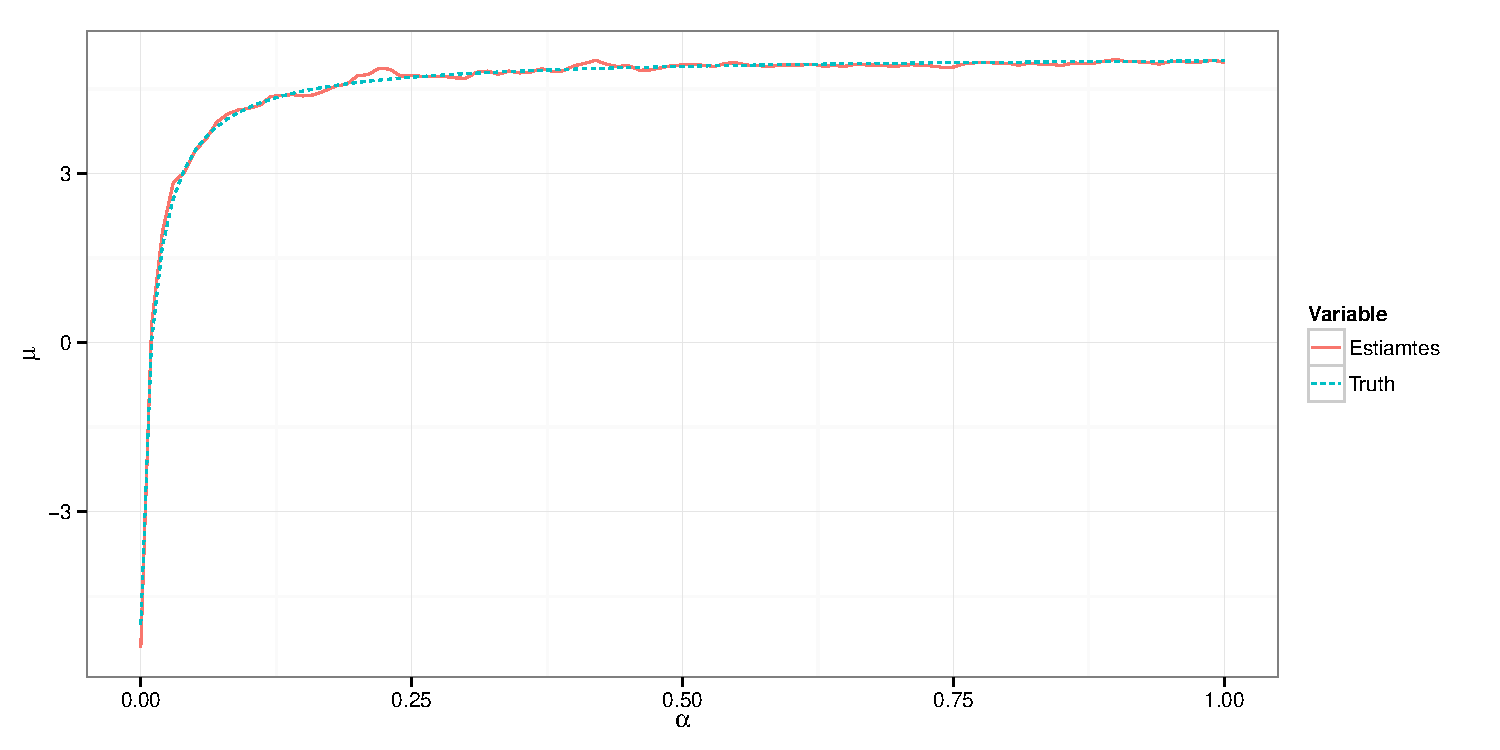
\includegraphics[width=\linewidth]{fig/mini_mu}
  \caption{The Monte Carlo estimates of the mean of the intermediate Normal
    distributions in the minimal example}
  \label{fig:mini mean}
\end{figure}

\begin{figure}
  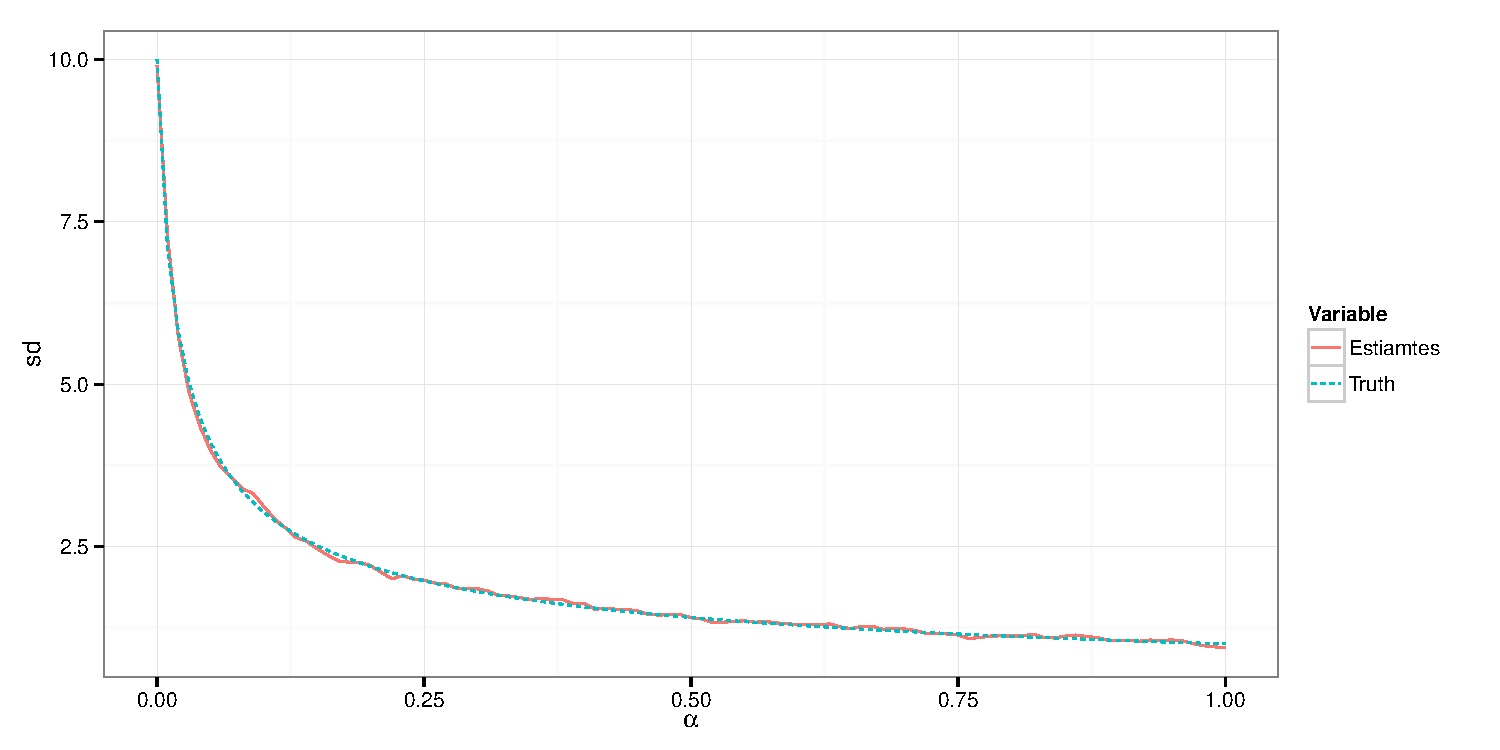
\includegraphics[width=\linewidth]{fig/mini_sd}
  \caption{The Monte Carlo estimates of the standard deviation of the
    intermediate Normal distributions in the minimal example}
  \label{fig:mini var}
\end{figure}

\section{Beyond the basics}
\label{sec:Beyond the basics}

The above example is quite minimal though it does show some advanced features
of the \vsmc library. In this section, we demonstrate the strength of the
presented framework by extend it with a few features. The first two shows that
it is trivial to implement the adaptive algorithms discussed in
section~\ref{sec:Extensions and refinements}. The third one shows that it is
easy to extend the framework with new algorithms, such as replacing the
built-in resampling algorithm.

\subsection{Implement the adaptive random walk scale}
\label{sub:Implement the adaptive random walk scale}

In the minimal example, we use the true standard deviation of the target
distribution for the Normal random walk. However, since we already implemented
a monitor that records the Monte Carlo estimates of the first and second raw
moments, it shall be trivial to use them to adaptively set the random walk
scales. To do this, we can use the \cppinline{pre_processor} member function
of the \cppinline{mini_move} class. Recall that, this member function is
called before any \cppinline{move_state} at each iteration. Here is the
modified \cppinline{mini_move} class,
\cppfile{code/mini_move_adaptive_scale.cpp}
The new class has a new member data \cppinline{sampler_}, which is a pointer
to the sampler. And through it, we can access the monitor named
\cppinline{"moments"}. The \cppinline{Monitor} class provides several ways to
read the record. Two of them are the overloaded \cppinline{record} member
function. It takes the index of the variable (starting with \cppinline{0}) as
its first argument. If no other arguments are provided, it simply returns the
most recent estimate. Alternatively, one can provide a second argument, which
shall be the iteration number. See the reference manual for details.

\subsection{Implement the CESS based adaptive schedule}
\label{sub:Implement the CESS based adaptive schedule}

To implement the \cess based adaptive schedule, again, we can use the member
function \cppinline{pre_processor} of the \cppinline{mini_move} class. In
\vsmc, the \cppinline{WeightSet} class provides the ability to compute the
value of $\cess/N$ (scaled to $[0,1]$) given (log) incremental weights. Below
is the modified \cppinline{mini_move} class,
\cppfile{code/mini_move_adaptive_schedule.cpp}
Now we have a member data \cppinline{alpha_}, which are simply indexed by the
iteration number. Inside member function \cppinline{pre_processor}, we make
sure that the first element is always $0$ and the last one is $1$. For any
value in between, we use a binary search to find the value that produce a new
target distribution with $\cess/N$ equal to a preset value $\cess^*/N$, which
we hard coded here as \cppinline{cess_star}. The call to
\cppinline{WeightSet::cess} takes an input iterator as its first argument, and
a boolean value, which indicate whether the incremental weights are on log
scale as its second argument. Now the \cppinline{alpha} member function no
longer compute $\alpha(t/T) = t/T$, instead it simply lookup in the vector
\cppinline{alpha_}.

\subsection{Use a new resampling algorithm}
\label{sub:Use a new resampling algorithm}

There are many areas of \vsmc algorithm been actively developed. Some of them
can be easy implemented with \vsmc through somehow ``creative'' use of the
classes like \cppinline{mini_move}, as demonstrated above. Other algorithms
may need to change \vsmc's internal. For example, \vsmc provide several
built-in resampling algorithms, which can be chosen through the constructor of
\cppinline{Sampler}. For example,
\begin{cppcode}
Sampler<mini> sampler(N, vsmc::Systematic);
\end{cppcode}
will construct a sampler with systematic resampling instead of the default
stratified resampling. Now consider that one has developed a new resampling
algorithm, to use it, one only need to define a function (or functor) similar
to the following,
\cppfile{code/resample.cpp}
where the input parameter \cppinline{N}, \cppinline{rng} and
\cppinline{weight} are the number of particles, an \cppoo{} \rng engine, and
the normalized weights, respectively. The output parameter
\cppinline{replication} shall be the number of replicates of each particle
after the resampling. To use it instead of one of the built-in algorithm, one
simply construct a sampler like the following,
\begin{cppcode}
Sampler<mini> sampler(N, resalg);
\end{cppcode}
Many advanced algorithms, including some recent development on parallel
resampling, are also possible though unavoidably, they will involve more
advanced \cpp techniques, which is beyond the scope of this chapter. See the
reference manual for details.

\section{Performance benchmark}
\label{sec:Performance benchmark}

One of the main motivation behind the creation of \vsmc is to ease the
parallelization with different programming models. The same implementation can
be used to built different samplers based on what kind of parallel programming
model is supported on the users' platforms. In this section we compare the
performance of various \smp parallel programming models and \opencl
parallelization. We use the Gaussian mixture model with \smc[2] algorithm as
shown in section~\ref{sub:Gaussian mixture model}. For a complete
documentation on its implementation with \vsmc, see \cite{software:VSMC}.

\subsection{Using the \protect\smp module}
\label{sub:Using the SMP module}

We consider five different implementations supported by \icpc~2013:
sequential, \tbb, \cilk, \openmp and \cppoo{} \cppinline{<thread>}. The
samplers are compiled with
\begin{makecode}
CXX=icpc -std=c++11 -gcc-name=gcc-4.7 -gxx-name=g++-4.7
CXXFLAGS=-O3 -xHost -fp-model precise  \
         -DVSMC_HAS_CXX11LIB_FUNCTIONAL=1  \
         -DVSMC_HAS_CXX11LIB_RANDOM=1
\end{makecode}
on a Ubuntu~12.10 workstation with an Xeon~W3550 (3.06GHz, 4 cores, 8 hardware
threads through hyper-threading) \cpu. A four components model and $100$
iterations with a prior annealing scheme is used for all implementations. A
range of numbers of particles are tested, from $2^3$ to $2^{17}$.

For different number of particles, the wall clock time and speedup are shown
in Figure~\ref{fig:bench-smp-perf}. For $10^4$ or more particles, the
differences are minimal among all the programming models. They all have
roughly 550\% speedup. With smaller number of particles, \vsmc's \cppoo
parallelization is less efficient than other industry strength programming
models. However, with $1000$ or more particles, which is less than typical
applications, the difference is not very significant.

\begin{figure}
  \centering
  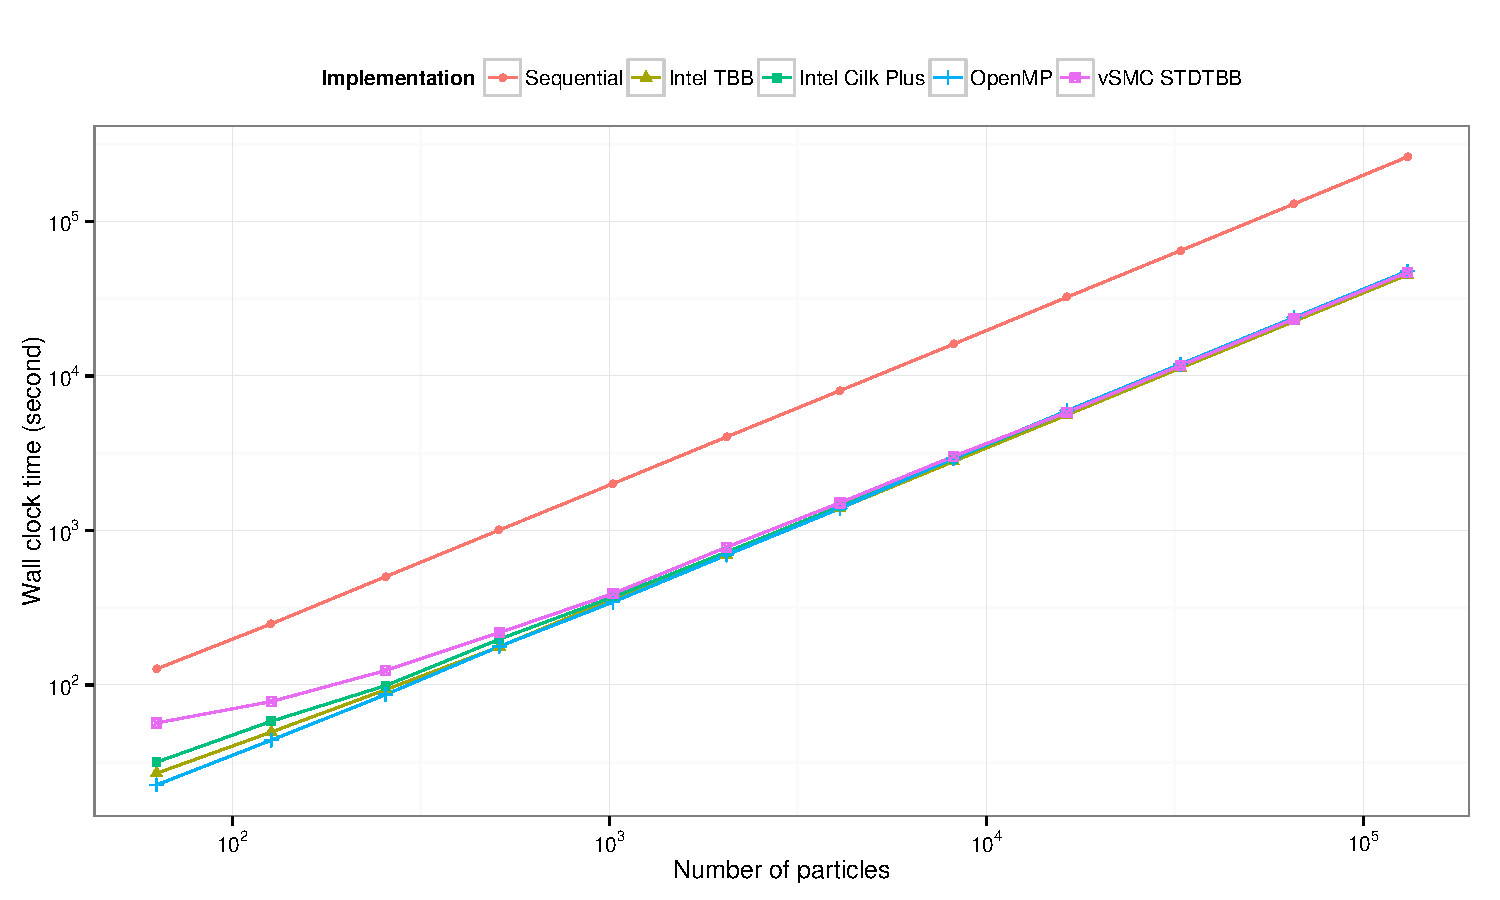
\includegraphics[width=\linewidth]{fig/bench-smp-time-running}
  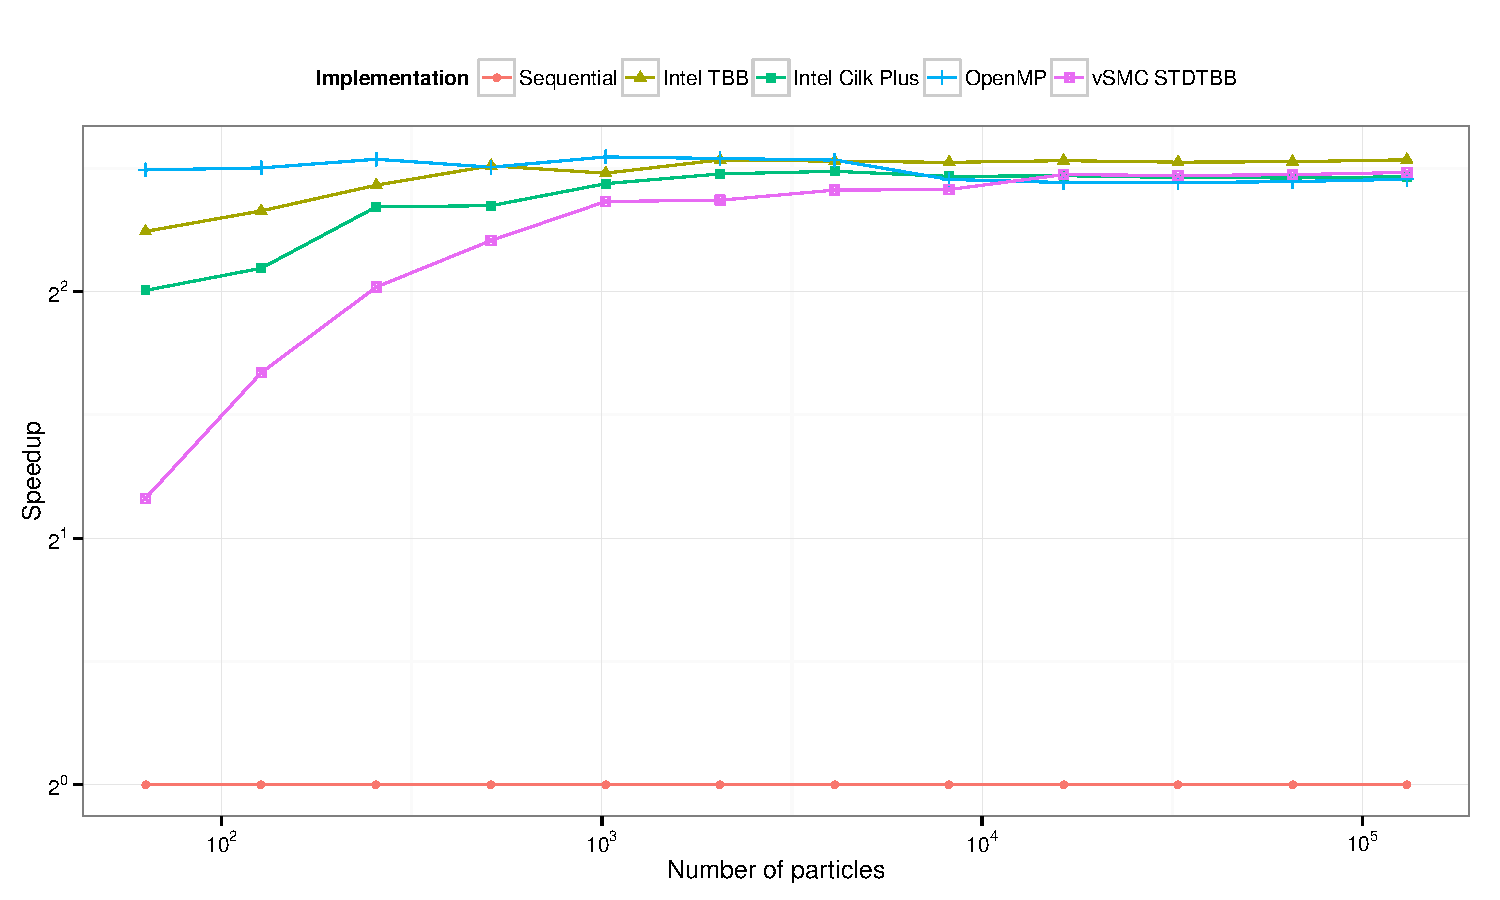
\includegraphics[width=\linewidth]{fig/bench-smp-speedup-running}
  \caption{Performance of \cpp implementations of Bayesian modeling for
    Gaussian mixture model (Linux; Xeon W3550, 3.06GHz, 4 cores, 8 threads).}
  \label{fig:bench-smp-perf}
\end{figure}

\subsection{Using the \protect\opencl module}
\label{sub:Using the OpenCL module}

The implementation of the same algorithm using \opencl is quite similar to
those using the \smp module.

\opencl implementations are also compared on the same workstation, which also
has an NVIDIA Quadro 2000 graphic card. \opencl programs can be compiled to
run on both \cpu and \gpu. For \cpu implementation, there are \iocl and \aocl
platforms. We use the \tbb implementation as a baseline for comparison.  The
same \opencl implementation are used for all the \cpu and \gpu runtimes.
Therefore they are not particularly optimized for any of them. For the \gpu
implementation, in addition to double precision, we also tested a single
precision configuration. Unlike modern \cpu, which have the same performance
for double and single precision floating point operations (unless \simd
instructions are used, which can have at most a speedup by a factor of 2),
\gpu penalize double precision performance heavily.

For different number of particles, the wall clock time and speed up are
plotted in Figure~\ref{fig:bench-ocl-perf}. With smaller number of particles,
the \opencl implementations have a high overhead when compared to the \tbb
implementation. With a large number of particles, \aocl has a similar
performance as the \tbb implementation. \iocl is about 40\% faster than the
\tbb implementation. This is due to more efficient vectorization and compiler
optimizations. The double precision performance of the NVIDIA \gpu has a 220\%
speedup and the single precision performance has near 1600\% speedup. As a
rough reference for the expected performance gain, the \cpu has a theoretical
peak performance of 24.48 GFLOPS. The \gpu has a theoretical peak performance
of 60 GFLOPS in double precision and 480 GFLOPS in single precision. This
represents 245\% and 1960\% speedup compared to the \cpu, respectively.

\begin{figure}
  \centering
  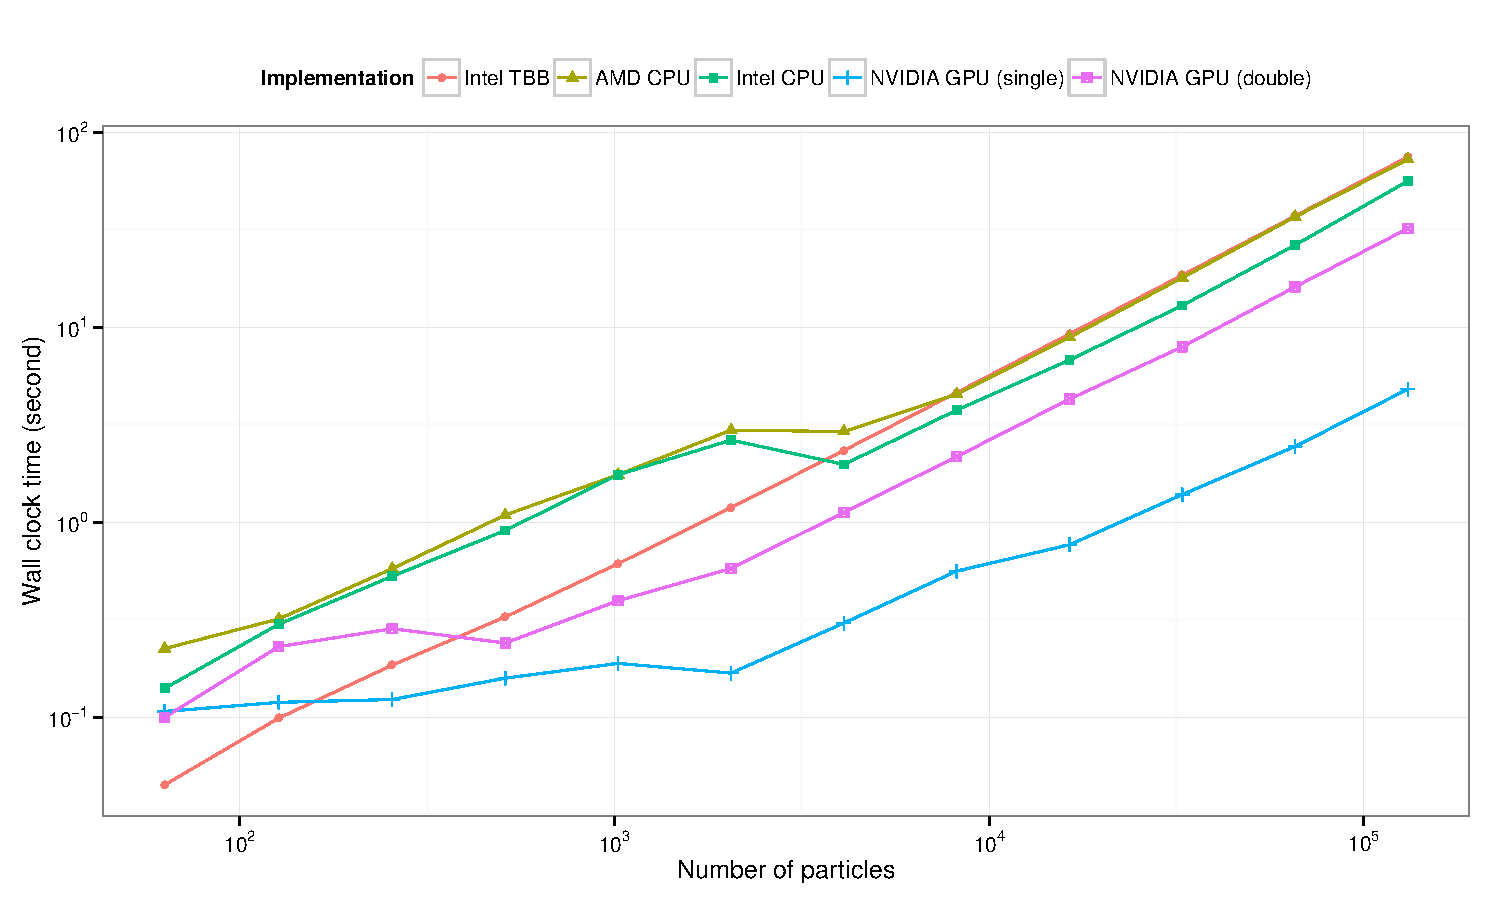
\includegraphics[width=\linewidth]{fig/bench-ocl-time-running}
  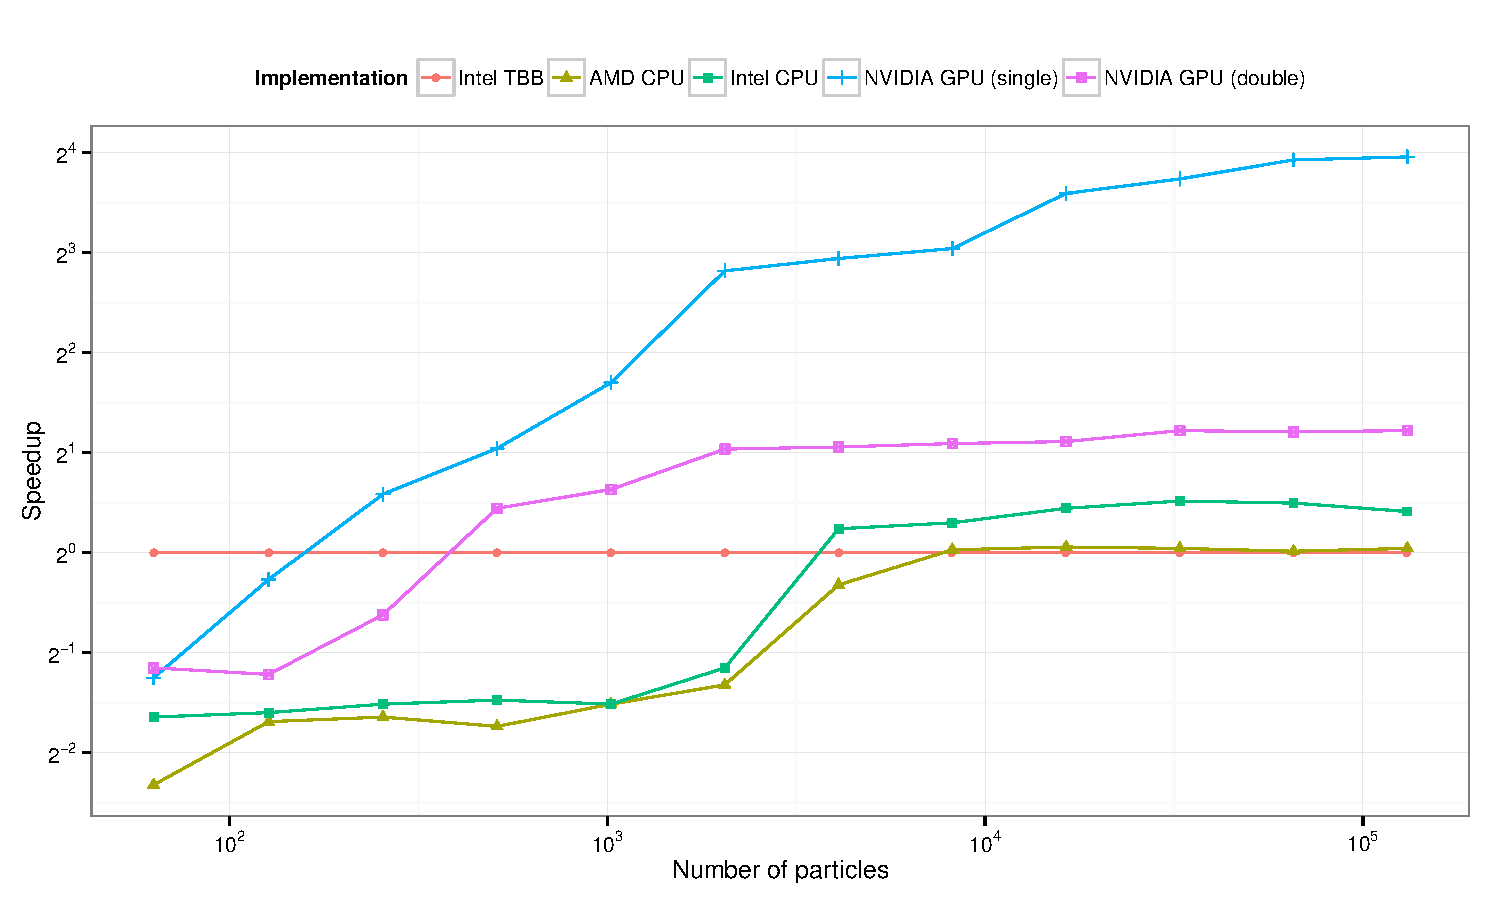
\includegraphics[width=\linewidth]{fig/bench-ocl-speedup-running}
  \caption{Performance of \opencl implementations of Bayesian modeling for
    Gaussian mixture model (Linux; Xeon W3550 \gpu, 3.06GHz, 4 cores, 8
    threads; NVIDIA Quadro 2000).}
  \label{fig:bench-ocl-perf}
\end{figure}

It is widely believed that \opencl programming is tedious and hard. However,
\vsmc provides facilities to manage \opencl platforms and devices as well as
common operations. Limited by the scope of this paper, the \opencl
implementation (distributed with the \vsmc source) is not documented in this
paper. Overall the \opencl implementation has about 800 lines including both
host and device code. It is not an enormous increase in effort when compared
to the 500 lines \smp implementation. Less than doubling the code base but
gaining more than 15 times performance speedup, we consider the programming
effort is relatively small.
